% Precondition:
% cd /home/gerald/van_development/van/aa
% cp /home/gerald/van_development/van/edu/latex/emoji.sty 
% 
% Build rules:
% pdflatex -shell-escape dia.tex
% evince dia.pdf

% This is the preamble of a LaTeX source code.
\documentclass[10pt,a4paper]{article}

% Import a package for a specific purpose: see https://www.ctan.org/
\usepackage[textwidth=17cm,textheight=26cm]{geometry}  % Customize the page layout.
\usepackage{tikzsymbols}    % Various emoticon, cooking symbols and trees.
\usepackage{enumitem}       % Control layout of itemize, enumerate, description.
\usepackage{wasysym}        % Provide symbols like \XBox.
\usepackage{scrextend}      % KOMA-Script class: labeling .
\usepackage{mdframed}       % Breakable framed and coloured boxes: mdframed.
\usepackage{anyfontsize}    % Select any font size: see \square.
\usepackage{stix}           % Complete set of mathematical glyphs: \boxtimes.
\usepackage[ngerman]{babel} % German orthography.
\usepackage{etoc}           % Table of contents control: \addcontentsline.
\usepackage{pdfpages}       % Inclusion of external PDF document: \includepdf.


% All paragraphs are without indentation.
\setlength{\parindent}{0pt}%

% Print a citiation right aligned.
\newcommand{\motto}[2]{%
  \hfill
  \begin{minipage}{0.33\textwidth}
    \small{} #1 \\
    \hspace*{\fill} #2
  \end{minipage}
  \topvskip\topvskip
}

% Introduce a paragraph section with a number.
\renewcommand{\theparagraph}{\arabic{paragraph}.}

% Force the numbering of a paragraph text.
\setcounter{secnumdepth}{4}

% Settings for a sub paragraph segment.
% Increment the sub paragraph counter.
% Print the sub paragraph title.
% Extend the contents.
\newcommand\p[1] {%
  \stepcounter{paragraph}
  {\large\bf\theparagraph \hskip 2pt \large\bf #1 \ \hskip -8pt}
  \addcontentsline{toc}{section} {\theparagraph\hskip 3pt #1}
}

% Subparagraph counters.
\newcounter{subc}
\renewcommand{\thesubc}{\arabic{subc}.}

\newcounter{subsubc}
\renewcommand{\thesubsubc}{\arabic{subsubc}.}

% Settings for a sub paragraph segment.
% Increment the sub paragraph counter.
% Print the sub paragraph title.
% Extend the contents.
\newcommand\subp[1] {%
  \stepcounter{subc}
  {\bf\theparagraph\thesubc}\hskip 3pt\rm #1\hskip 4pt
  \addcontentsline{toc}{subsection}{\theparagraph\thesubc\hskip 3pt #1}
}

% Settings for a sub sub paragraph segment.
% Increment the sub sub paragraph counter.
% Print the sub sub paragraph title.
% Extend the contents.
\newcommand\subsubp[1] {%
  \stepcounter{subsubc}
  {\bf\theparagraph\thesubc\thesubsubc}\hskip 3pt\rm #1\hskip 4pt
  \addcontentsline{toc}{subsubsection}{\theparagraph\thesubc\thesubsubc\hskip 3pt #1}
}

% Elements of a title page.
\newcommand\svthema{Diagnose}
\newcommand\svperson{Gerald Schüller}
\newcommand\svdatum{\today}


% Color list:
\definecolor{alizarin}{rgb}{0.82, 0.1, 0.26}
\definecolor{amber(sae/ece)}{rgb}{1.0, 0.49, 0.0}
\definecolor{amethyst}{rgb}{0.6, 0.4, 0.8}
\definecolor{aqua}{rgb}{0.0, 1.0, 1.0}
\definecolor{aquamarine}{rgb}{0.5, 1.0, 0.83}
\definecolor{burntorange}{rgb}{0.8, 0.33, 0.0}
\definecolor{darkbrown}{rgb}{0.4, 0.26, 0.13}
\definecolor{english}{rgb}{0.0, 0.5, 0.0}
\definecolor{indigo(web)}{rgb}{0.29, 0.0, 0.51}
\definecolor{midnightblue}{rgb}{0.1, 0.1, 0.44}


% Document and protocol track
\newcommand\expt[1] {{\color {darkbrown} {\bf #1}}}       % Experiment
\newcommand\info[1] {{\color {midnightblue} {\bf #1}}}    % Informatoin

\newcommand\prop[1] {{\color {alizarin} {\bf #1}}}        % Proposal
\newcommand\draf[1] {{\color {amber(sae/ece)} {\bf #1}}}  % Draft
\newcommand\rele[1] {{\color {english} \bf {#1}}}         % Release
\newcommand\rewo[1] {{\color {aqua} {\bf #1}}}            % Rework

\newcommand\emps[1] {{\color {indigo(web)} {\bf #1}}}     % Emphasis

\newcommand\opti[1] {{\color {amethyst} {\bf #1}}}        % Optional
\newcommand\mand[1] {{\color {burntorange} {\bf #1}}}     % Mandatory


% Frame list style of a single day.
\mdfdefinestyle{daystyle}{%
  skipabove=4pt,
  skipbelow=0pt,
  %  leftmargin=-16pt,
  leftmargin=-10pt,
  topline=false,
  bottomline=false,
  leftline=false,
  rightline=false
}

% Preceeding vertical skip of a paragramph.
\newcommand\topvskip {\vskip 8pt}

% Preceeding horizontal skip of a minipage.
\newcommand\tophskip {\hskip -14pt}

% Horizontal dividing line between two days.
\newcommand\ddivide {\vskip -9pt \hrule \vskip 6pt}

% First and last horizontal dividing line of a week.
\newcommand\fdivide {\vskip  6pt \hrule \vskip 6pt}
\newcommand\ldivide {\vskip -9pt \hrule \hrule \hrule \vskip 8pt}

% Set of natural numbers.
\newcommand{\N}{\mathbb{N}}

% Numbering of the day entries.
\newcommand\n[1] { {\sl #1.} \hskip 5pt }


% Start of a LaTeX text, that is to be printed.
\begin{document}

% Front page
\title{ \textbf{\color{blue}\svthema} \Springtree [1.5] }
\author{ \textsl{\color{red}\svperson} --- \svdatum }
\date{}

% You tell LaTeX the information used to produce the title page.
\maketitle

\motto{Der Fliege den Ausweg aus dem Fliegenglas zeigen.}{L. Wittgenstein, PU, 309.}

% Generate the table of contents.
\tableofcontents

% Generate the apendix table.
\appendix

\newpage
\p{{\info {Document-Track}}}

% Initialize the subparagraph counters.
\setcounter{subc}{0}

\topvskip
\begin{minipage}{0.90\textwidth} 
  \begin{labeling}{Information:} 
    \setlength\itemsep{-3pt}
  
  \item[Experiment:]  \textbackslash {\expt {expt}}
  \item[Information:] \textbackslash {\info {info}}
  \item[Proposal:]    \textbackslash {\prop {prop}}
  \item[Draft:]       \textbackslash {\draf {draf}}
  \item[Release:]     \textbackslash {\rele {rele}}
  \item[Rework:]      \textbackslash {\rewo {rewo}}
  \item[Emphasis:]    \textbackslash {\emps {emps}}
  \end{labeling}
\end{minipage}


\topvskip
\p{\rele {Anamnese}}

% Initialize the subparagraph counters.
\setcounter{subc}{0}

\topvskip
\subp{\info {Bibliographie}}

\topvskip
\verb+https://de.wikipedia.org/wiki/Alkoholkrankheit+ \\
\verb+https://de.wikipedia.org/wiki/Psychotrope_Substanz+ \\
\verb+https://de.wikipedia.org/wiki/Psyche+ \\
\verb+https://www.wittgensteinproject.org/w/index.php?title=+ \\
\verb+Philosophische_Untersuchungen#+ \\
\verb+https://de.wikipedia.org/wiki/Ethanol+ \\
\verb+https://www.dimdi.de/static/de/klassifikationen/icd/icd-10-who/+ode-suche/htmlamtl2019/+

\topvskip
% Command for \
\verb+https://de.wikibooks.org/wiki/LaTeX-Kompendium:_Sonderzeichen+ \\
% Kästchen zum ankreuzen automatisch multipli choise.
\verb+https://golatex.de/viewtopic.php?t=5926+ \\
\verb+https://tex.stackexchange.com/questions/163986/format-table-of-contents-with-latex+ \\
\verb+https://tex.stackexchange.com/questions/101538/+ \\
\verb+addcontentsline-lines-added-to-toc-not-numbered-and-lines-added-to-tot-not-sh+ \\
\verb+https://tex.stackexchange.com/questions/176173/appendix-adding-pdf+


\topvskip
\subp{\info {Definitionen}}

% Initialize the subparagraph counters.
\setcounter{subsubc}{0}

\topvskip
\tophskip
\begin{minipage}{0.90\textwidth}  
  \begin{itemize}
    \setlength\itemsep{-3pt}
    
  \item {\emps {Alkoholkrankheit}} ist die Abhängigkeit von der psychotropen
    Substanz Ethanol bzw. Alkohol.
    
  \item {\emps {Psychotrope Substanz}} ist ein Wirkstoff, der die menschliche
    Psyche beeinflusst.

  \item {\emps {Psyche}} ist die Gesamtheit aller geistigen Eigenschaften wie
    Denken, Lernen, Emotionen - Entspannung, Erleichterung, Euphorie $\ldots$ -,
    Wahrnehmen, Empfinden - Tastempfindung, Atmen, Handhaltung, $\ldots$ - ,
    Empathie, Wissen, Intuition und Motivation.

  \end{itemize}
\end{minipage}


\topvskip
\subp{\rele {Symptome}}

% Initialize the subparagraph counters.
\setcounter{subsubc}{0}

\vskip 4pt
Jeden Tag kaufe ich ein bis zwei Flaschen Wein und trinke meist ab dem
späten Nachmittag oder eher selten ab Mittag solange, bis ich einschlafe. Meine
früheren Interessen wie Sport, Treffen mit Freunden $\ldots$ habe ich aufgegeben
ausser Programmieren verknüpft mit Trinken. Wenn ich nicht trinke, bin ich
ungeduldig und wortkarg.


\topvskip
\subp{\rele {Klassifikation nach ICD-10}}

% Initialize the subparagraph counters.
\setcounter{subsubc}{0}

\topvskip
\subsubp{\rele {Abhängigkeitssyndrom}}

\topvskip
\tophskip
\begin{minipage}{0.90\textwidth}
  
  \begin{enumerate}[label={\Square}]
    \setlength\itemsep{-3pt}
  
  \item [\XBox] Zwanghaftes Verlangen, Alkohol zu konsumieren
  \item [\XBox] Verminderte Kontrollfähigkeit bei der Menge
  \item Körperliche Entzugserscheinungen
  \item [\XBox] Nachweis einer Toleranz: zunehmend größere Mengen an Alkohol
  \item [\XBox] Einengung des Denkens auf Alkohol
  \item [\XBox] Anhaltender Substanzkonsum trotz gesundheitlicher und sozialer
    Folgeschäden
    
  \end{enumerate}
  
\end{minipage}

\topvskip
Abhängigkeitssyndrom (F10.2) trifft bei mir zu, da mehr als zwei Kriterien mindestens einen
Monat lang gleichzeitig vorhanden sind.


\topvskip
\subsubp{\rele {Akute Alkoholintoxikation (akuter Alkoholrausch)}}

\vskip 4pt
Eine akute Alkoholintoxikation (F10.0) trifft bei mir zu, da folgende
Verhaltensauffälligkeiten und Merkmale vorliegen:

\topvskip
\tophskip
\begin{minipage}{0.90\textwidth}
  
  \begin{itemize}
    \setlength\itemsep{-3pt}
  
  \item Enthemmung
  \item Aufmerksamkeitsstörung
  \item Einschränkung der Urteilsfähigkeit
  \item verwaschene Sprache
  \item Gesichtsröte (Erröten)
    
  \end{itemize}
  
\end{minipage}


\topvskip
\subp{\rele {Klassifikation nach DSM-5}}

% Initialize the subparagraph counters.
\setcounter{subsubc}{0}


\topvskip
\subsubp{\rele {Störung durch Alkoholkonsum (Alkoholkonsumstörung)}}

\topvskip
\tophskip
\begin{minipage}{0.90\textwidth}
  
  \begin{enumerate}[label={\Square}]
    \setlength\itemsep{-3pt}
  
  \item [\XBox] Alkohol wird in größeren Mengen oder länger als beabsichtigt
    konsumiert.
  \item [\XBox] erfolglose Versuche, den Alkoholkonsum zu verringern oder zu
    kontrollieren    
  \item [\XBox] hoher Zeitaufwand, um Alkohol zu beschaffen, zu konsumieren oder
    sich zu erholen
  \item [\XBox] Craving oder ein starkes Verlangen, Alkohol zu konsumieren
  \item [\XBox] Alkoholkonsum verbunden mit der Nicht-Erfüllung von
    Verpflichtungen: Arbeit und zu Hause
  \item [\XBox] Alkoholkonsum trotz ständiger sozialer oder zwischenmenschlicher
    Probleme
  \item [\XBox] soziale, berufliche oder Freizeitaktivitäten werden aufgrund des
    Alkoholkonsums aufgegeben
  \item Alkoholkonsum verbunden mit einer körperlichen Gefährdung
  \item [\XBox] Alkoholkonsum trotz Kenntnis eines anhaltenden oder
    wiederkehrenden psychischen Problems
  \item [\XBox] Toleranzentwicklung mit Dosissteigerung und verminderter Wirkung
  \item Entzugssymptome
    
  \end{enumerate}
\end{minipage}

\topvskip
Alkoholkonsumstörung trifft bei mir zu, da mehr als ein Kriterium über zwölf
Monate vorliegt.

\vskip 4pt
Der Schweregrad ist schwer, da mehr als 5 Symptomkriterien erfüllt sind.


\topvskip
\subp{\rele {Krankheitsverlauf und -bild}}

% Initialize the subparagraph counters.
\setcounter{subsubc}{0}

\topvskip
\subsubp{\rele {Krankheitsverlauf}}

\vskip 4pt
Aktuell befinde ich mich wohl im Übergang von der kritischen zur chronischen
Phase.

\begin{labeling}{{\bf Chronische Phase:}} 
  \setlength\itemsep{-3pt}
  
\item[{\emps {Kritische Phase:}}]  Der Alkoholiker kann sein Trinken nun
  überhaupt nicht mehr kontrollieren. $\ldots$
  
\item[{\emps {Chronische Phase:}}] Der Alkohol beherrscht den Trinker nun
  vollkommen. Seine Persönlichkeit verändert sich. Er trinkt unter der Woche, am
  hellen Tag, häufig schon ab Mittag.  $\ldots$

\end{labeling}

\vskip 0pt
\subsubp{\rele {Ausprägungen der Krankheit}}

\vskip 4pt
Selbst würde ich mich einschätzen als {\emps {Gamma-Typ}} (Rauschtrinker, Alkoholiker),
denn ich trinke täglich. Typisch ist der Kontrollverlust: ich kann nicht
aufhören zu trinken bis ich einschlafe.


\topvskip
\subp{\rele {Biologie der Alkoholsucht}}

% Initialize the subparagraph counters.
\setcounter{subsubc}{0}

\vskip 4pt
Alkohol verändert im Gehirn Rezeptoren, die bei mir die Entspannung verbessern. Wegen
deren Anpassung erhöhe ich die Alkoholmenge. \\
Mit Alkohol wird vermehrt Dopamin und Endorphine produziert. \\
Dopamin ist ein Hormon, das die Motivation fördert. \\
Endorphine sind körpereigene Opioide, die u.a. eine Euphorie hervorrufen.


\vskip 4pt
\subp{\rele {Krankheitsursachen}}

% Initialize the subparagraph counters.
\setcounter{subsubc}{0}

\topvskip
\subsubp{\rele {Genetische Faktoren}}

\vskip 4pt
Meine Mutter war tablettensüchtig und vermutlich gibt es bei mir eine angeborene
Alkoholverträglichkeit.


\topvskip
\subsubp{\rele {Psychologische Faktoren}}

\vskip 4pt
Die schnell eintretenden positiven Wirkungen des Alkohols wie Entspannung und
Glücksgefühle wie Euphorie, Zufriedenheit - Stolz, $\ldots$ -  verstärken das
Suchtverhalten.


\topvskip
\subp{\rele {Rückfall}}

% Initialize the subparagraph counters.
\setcounter{subsubc}{0}

\vskip 4pt
Wenn ich mich nicht total abstinent verhalte, erwarte ich einen
{\bf schweren} {\bf Rückfall} {\bf (relapse)} in alte Trink\-muster, die sich
auf Alkoholmenge, Trinkfrequenz und Trinkdauer beziehen.


\newpage
\p{\expt {Diagnose}}

% Initialize the subparagraph counters.
\setcounter{subc}{0}


\topvskip
\subp{\info {Bibliographie}}

% Initialize the subparagraph counters.
\setcounter{subsubc}{0}

\topvskip
\verb+https://de.wikipedia.org/wiki/Diagnose+ \\
\verb+https://de.wikipedia.org/wiki/Medizinische_Dokumentation+ \\
\verb+https://de.wikipedia.org/wiki/Anamnese+ \\
\verb+https://de.wikipedia.org/wiki/%C3%84tiologie_(Medizin)+ \\
\verb+https://de.wikipedia.org/wiki/Pathogenese+ \\
\verb+https://de.wikipedia.org/wiki/Labordiagnostik+ \\
\verb+https://de.wikipedia.org/wiki/ICD-10+ \\
\verb+https://www.icd-code.de/suche/icd/recherche.html?sp=0&sp=SAlkoholkrankheit+


\topvskip
\subp{\expt {Labordiagnostik}}

% Initialize the subparagraph counters.
\setcounter{subsubc}{0}


\topvskip
\subsubp{\info {Bibliographie}}

\topvskip
\verb+https://de.wikipedia.org/wiki/Blutbild+ \\
xxx \\
\verb+https://www.blutwert.net/+ \\
\verb+https://www.medpertise.de/blutwerte/blutbild/mch/zu-hoch/+ \\
\verb+https://www.grossesblutbild.de/blutwerte-alkohol-abhaengigkeit.html#+ \\
\verb+Das_MCV_stellt_einen_wichtigen_Blutwert_dar+


\topvskip
\subsubp{\info {Definitionen}}

\topvskip
\tophskip
\begin{minipage}{0.90\textwidth}  
  \begin{itemize}
    \setlength\itemsep{-3pt}
  
  \item {\emps {Blutbild}} ist eine Zusammenstellung wichtiger Befunde aus einer Blutprobe.
    
  \end{itemize}
\end{minipage}


\topvskip
\subsubp{\expt {Blutbild}}


\topvskip
{\info {Leberwerte}}

% Initialize the subparagraph counters.
\setcounter{subsubc}{0}

Im Blut befinden sich die Enzyme {\bf GOT} oder {\bf ASAT} und {\bf GPT} oder
{\bf ALAT}, über die man den Zustand und die Aktivität der Leber erkennen kann.
Wenn diese Enzyme mit einer gewissen Konzentration im Blut vorkommen ist die
Leber beschädigt.

Unten ist die normal Konzentration der Enzyme aufgelistet: UL = Unit pro Liter.

% Bezeichnung  Normalwert_Mann 
% GOT (ASAT)       bis 50 U/l
% GPT (ALAT)       bis 50 U/l



\topvskip
\subsubp{\expt {12.09.2022}}

\vskip 4pt
Der Ery-Wert liegt unterhalb der unteren Schwelle und der MCH- und MCV-Wert
überschreiten die obere Schranke.

\vskip 4pt
Zu wenig Erythrozyten deuten auf eine Anämie (Blutarmut) hin. Eine
Mangelerscheinung könnte die Ursache der Anämie sein wie Eisenmangel oder
Vitaminmangel.

\vskip 4pt
Die häufigste Ursache für einen zu hohen MCH-Wert ist Vitamin-B12-Mangel und
Folsäuremangel wegen unzureichender Zufuhr mit der Nahrung.

\vskip 4pt
Ist der MCV zu hoch, dann sind die roten Blutkörperchen zu groß. Häufigste
Ursachen sind ein Vitamin-B12-Mangel oder ein Folsäuremangel.
Übermäßiger Alkoholkonsum führen ebenfalls zu erhöhten MCV-Werten.
Der Wert steigt an, sobald die Patienten pro Tag mehr als 60 Gramm Alkohol
konsumieren. 1 Glas Wein (100 ml, 11 Vol.-\%): \\
$100 ml \times (11 \div 100) \times 0.8 = 8,8 g$ Alkohol.


\topvskip
\p{{\expt {Auswertung}}}

% Initialize the subparagraph counters.
\setcounter{subc}{0}


\topvskip
\p{{\info {Protokoll-Track}}}

% Initialize the subparagraph counters.
\setcounter{subc}{0}

\topvskip
\begin{minipage}{0.90\textwidth}  
  \begin{labeling}{Mandatory list elements:} 
    \setlength\itemsep{-3pt}
  
  \item[Mandatory list elements:]  \textbackslash {\mand {mand}}
  \item[Optional list elements:]   \textbackslash {\opti {opti}}

  \end{labeling}
\end{minipage}


\topvskip
\subp{\info {Bibliographie}}

% Initialize the subparagraph counters.
\setcounter{subsubc}{0}

\topvskip
\verb+https://de.wikipedia.org/wiki/Therapie+ \\
\verb+https://de.wikipedia.org/wiki/Monitoring+ \\
\verb+https://de.wikipedia.org/wiki/Protokoll_(Niederschrift)+ \\
\verb+https:https://de.wikipedia.org/wiki/Gem%C3%BCt+ \\
\verb+https://de.wikipedia.org/wiki/Selbsthilfegruppe+ \\
\verb+https://www.anonyme-alkoholiker.at/images/E-Medien/2021-docs/+ \\
\verb+2021_09%20-%20SMZ%20Liebenau.pdf+ \\
\verb+https://guttempler.org/+ \\
\verb+https://www.herzstiftung.de/ihre-herzgesundheit/das-herz/welcher-puls-ist-normal+ \\
\verb+https://www.herzstiftung.de/ihre-herzgesundheit/gesund-bleiben/bluthochdruck/+ \\
\verb+was-ist-bluthochdruck+ \\
\verb+https://de.wikipedia.org/wiki/Men%C3%BC_(Speisenfolge)+ \\
\verb+https://de.wikipedia.org/wiki/Intermittierendes_Fasten+

\topvskip
\verb+https://tex.stackexchange.com/questions/116101/add-bold-enumerate-items+ \\
\verb+https://tex.stackexchange.com/questions/58087/+ \\
\verb+https://www.physicsread.com/latex-square-symbol/+ \\
\verb+how-to-remove-the-warnings-font-shape-ot1-cmss-m-n-in-size-4-not-available+ \\
\verb+https://tex.stackexchange.com/questions/50804/explicit-space-character+


\topvskip
\subp{\info {Definitionen}}

% Initialize the subparagraph counters.
\setcounter{subsubc}{0}

\topvskip
\tophskip
\begin{minipage}{0.90\textwidth}  
  \begin{itemize}
    \setlength\itemsep{-3pt}

  \item {\emps {Monitoring}} Monitoring ist die Überwachung von Vorgängen.
  
  \item {\emps {Protokoll}} ist eine Aufzeichnung, in der Zeitpunkt von
    Zuständen und Vorgänge aufgelistet werden.

  \item {\emps {Gemütszustand}} ist das aktuelle psychische Befinden eines
    Menschen.

  \item {\emps {Puls}}, normalerweise Herfrequenz, ist die Bewegung des Blutes
    pro Minute, Pulswelle, das bei jedem Herzschlag gegen die Arterienwände
    gedrückt wird.

  \item {\emps {Blutdruck}} ist der Druck, den das Blut auf die Wand von
    Arterien und Venen ausübt. Der systolische Wert ist der Druck, mit dem das
    Herz das Blut pumpt (Systole). Der diastolische Wert ist der niedrigste
    Druck vor der nächsten Herzkontraktion, also wenn der Herzmuskel sich wieder
    mit Blut gefüllt hat (Diastole). Der Blutdruck hängt von dem Druck ab, mit
    dem das Herz das Blut in den Kreislauf pumpt und von der Elastizität und dem
    Durchmesser der Gefäße.

  \item {\emps {Menü}} Als Menü ist eine Kombination von Speisen und Gerichten,
    die aus mehreren Gängen besteht.
    
  \item {\emps {Intervallfasten}} ist eine Ernährungsform mit einer konstanten
    Fastenzeit zwischen der letzten und ersten Nahrungsaufnahme.
    
  \item {\emps {Selbsthilfegruppe}} oder {\emps {SHG}} ist ein
    selbstorganisiertes Treffen von Menschen, die ein gleiches Problem haben wie
    Alkoholkrankheit.
    
  \item {\emps {Anonyme Alkoholiker}} oder {\emps {AA}} ist eine
    Selbsthilfegruppe für Alkoholiker mit dem Vorsatz:
    ,,Nur heute, 24 Stunden lang, lasse ich das erste Glas stehen.''
    
  \item {\emps {Guttempler}} ist eine Selbsthilfegruppe, die erwartet, dass man
    weder Alkohol noch andere bewußtseinsverändernde Drogen konsumiert.
    
  \end{itemize}
\end{minipage}

\topvskip
\subp{\info {Gefühlszustände}}

% Initialize the subparagraph counters.
\setcounter{subsubc}{0}

\topvskip
\verb+https://de.wikipedia.org/wiki/Emoticon+

\topvskip
Emoticon sind Zeichen, mit denen man Stimmungs- oder Gefühlszustände ausdrückt.

\topvskip
\begin{labeling}{{\mand {-1.5:}}}
  \setlength\itemsep{-3pt}
  \item[-2:]   \dChangey [1.5][yellow]{-2}
  \item[-1.5:] \dChangey [1.5][yellow]{-1.5}
  \item[-1:]   \dChangey [1.5][yellow]{-1}
  \item[0:]    \dChangey [1.5][yellow]{0}
  \item[1:]    \dChangey [1.5][yellow]{1}
  \item[1.5:]  \dChangey [1.5][yellow]{1.5}
  \item[2:]    \dChangey [1.5][yellow]{2}
\end{labeling}


\topvskip
\p{{\rele {Alltagsstruktur}}}

% Initialize the subparagraph counters.
\setcounter{subc}{0}

\definecolor{arylideyellow}{rgb}{0.91, 0.84, 0.42}

\topvskip
$AS = [ C, B, A, M, K, E, H, Z, P, SHG, F, V, W, G, L, T, S ]$

\begin{mdframed}[style=daystyle]
  \begin{labeling}{{\mand {$SHG :=$}}}
    \setlength\itemsep{-3pt}
  \item[$C :=$ ]   Countdown: verfügbare Zeit
  \item[$B :=$ ]   Befinden oder Stimmung
  \item[$A :=$ ]   Abstinenz in Tagen
  \item[$M :=$ ]   Monitoring der Gesundheit: Ruhepuls und Blutdruck
  \item[$K :=$ ]   Körperpflege: Zähne putzen, Duschen
  \item[$E :=$ ]   Essen: Obst, Gemüse, $\dots$
  \item[$H :=$ ]   Snoopy
  \item[$Z :=$ ]   Zazen oder Meditaion
  \item[$P :=$ ]   Physische Zustand: Intervallfasten, Gymnastik, Laufen
  \item[$SHG :=$ ] Selbsthilfegruppen: AA, Guttempler, Meditationsgruppe
  \item[$F :=$ ]   Freunde
  \item[$V :=$ ]   Verwaltung: Bank, Behörden, $\ldots$
  \item[$W :=$ ]   Wohnung: Staub saugen, Wäsche waschen, $\ldots$
  \item[$G :=$ ]   Garten: Rasen mähen, $\ldots$
  \item[$T :=$ ]   Tätigkeit, Arbeit oder Beruf
  \item[$L :=$ ]   Lesen
  \item[$S :=$ ]   Schlaf
\end{labeling}
\end{mdframed}

$n,i,j,k,l,m,n,o \in \N$

\fboxrule = 2pt % Sets the width of the frame.
\fboxsep  = 4pt  % Set the separation between the text and the frame.

\topvskip
\fcolorbox{arylideyellow}{white}{
  \begin{minipage}{0.95\textwidth}
    \begin{labeling}{{\mand {Körperpflege:}}}
      \setlength\itemsep{-3pt}
    \item[{\mand {Countdown:}}]    \n{\_} {\rewo {16 Stunden}}
    \item[{\mand {Stimmung:}}]     \n{\_} \dChangey [1.5][yellow]{0}
    \item[{\mand {Abstinenz:}}]    \n{\_} $i$ Tage
    \item[{\mand {Körperpflege:}}]  \n{n} $j \times$ Zähne putzen, $\square$ Duschen, $\square$ Frisör
    \item[{\mand {Gesundheit:}}]    \n{n} Ruhepuls: $k$ (70), Blutdruck: $l/m$ (89/143)
    \item[{\mand {Zazen:}}]         \n{n} $\square$ 25 min $\circ$ Kinin $\circ$ $\square$ 25 min
    \item[{\mand {Sport:}}]         \n{n} $n \times 2 \times 1\ min$ Schulterübungen (3); $\square$ Laufen: 3 km
    \item[{\mand {Essen:}}]         \n{n} 
      \vskip -14pt \hskip 20 pt
      \begin{minipage}{0.75\textwidth}  
        \begin{labeling}{$\square$ Fasten:} 
          \setlength\itemsep{-3pt}  
        \item[$\square$ Menü:]    17.00 - 18.00: $e \in Speisekarte$
        \item[$\square$ Obst:]             Apfel, Banane, $\ldots$
        \item[$\square$ Fasten:]  18.00 - 10.00
        \end{labeling}
      \end{minipage}
      \vskip 4pt
    \item[{\mand {Snoopy:}}]        \n{n} $o$ Spaziergänge (4); $\square$ SHG ohne Snoopy
    \item[{\mand {SHG:}}]           \n{n} $\square$ AA, Guttempler, Meditation
    \item[{\mand {Freunde:}}]       \n{n} $\square$ z.B. Frühstück
    \item[{\mand {Verwaltung:}}]    \n{n} $\square$ z.B. Finanzamt, Mikrozensus, Gewerbsteuer, Therapieformulare
    \item[{\mand {Haus:}}]          \n{n} $\square$ z.B. Staub saugen
    \item[{\mand {Garten:}}]        \n{n} $\square$ z.B Gras mähen
    \item[{\mand {Beruf:}}]        \n{\_} Aufschub bis nach der stationären Therapie
    \item[{\mand {Lesen:}}]         \n{n} $\square$ z.B. Wittgenstein (1 Std.)
    \item[{\mand {Schlaf:}}]        \n{n} $\square$ 22.00 - 06.00
    \item[{\opti {Hausarzt:}}]      \n{n} Dr. Haller: $\ldots$
    \item[{\opti {Beratung:}}]      \n{n} Frau Etter: $\ldots$
  \end{labeling}
  \end{minipage}
}

\topvskip
\p{{\rele {Speisekarte}}}

% Initialize the subparagraph counters.
\setcounter{subc}{0}

\topvskip
\verb+https://www.chefkoch.de/+

\fboxrule = 2pt % Sets the width of the frame.
\fboxsep  = 4pt  % Set the separation between the text and the frame.

\topvskip
\fcolorbox{aquamarine}{white}{
  \begin{minipage}{0.95\textwidth}
    \begin{enumerate}
      \setlength\itemsep{-3pt} 
    \item Geflügelwiener, Zwiebel, Champignons, Ravioli
    \item Geflügelwiener, Zwiebel, Champignons, Blumenkohl
    \item {\expt {Geflügelwiener - Scheiben -, Lauch, Mais, Paprika, Ketchup, Senf (Wurstgulasch)}}
    \item Hähnchen, Zwiebel, Champignons, Kohlrabi
    \item Hähnchen, Zwiebel, Champignons, Kartoffeln
    \item {\expt {Hähnchen, Paprika, Zucchini, Zwiebel, Champignons}}
    \item Leber (Milch, Mehl, 2/2/10 min), Zwiebel, Champignons, Reis
    \item {\expt {Leber - geschnezelt -, Zwiebel, Kartoffelpüree: Brühe, Muskat}}
    \item {\expt {Leber - Streifen -, Knoblauch, Peperoni, Petersilie, Kümmel, Chili, Zimt, Blumenkohlpüree: Brühe, Muskat (marokanisch)}}
    \item {\expt {Leber - Würfel- , Zwiebel, Knoblauch, Peperoni, Koriander, Kurkuma, Zucchinipüree: Brühe, Muskat (indisch)}}
    \item {\expt {Kassler, Sauerkraut, Kartoffelpüree: Brühe, Muskat}}
    \item {\expt {Thunfisch, Karotten, Erbsen, Zwiebel, Champignons, Couscous}}
    \item {\expt {Tofu, Zwiebel, Champignons, , Polenta}}
    \item {\expt {Schinken, Zwiebel, Paprika, Champignons, Ravioli}}
    \end{enumerate}    
  \end{minipage}
}

\topvskip
\p{{\rele {Protokoll}}}

% Initialize the subparagraph counters.
\setcounter{subc}{0}


\topvskip
\subp{\rele {KW 36}}

% Initialize the subparagraph counters.
\setcounter{subsubc}{0}

\topvskip
{\mand {Gewicht:}} -

\fdivide
{\rele {8.9.2022 - Donnerstag}}

\begin{mdframed}[style=daystyle]
  \begin{labeling}{{\mand {Stimmung:}}}
    \setlength\itemsep{-3pt}
  \item[{\mand {Stimmung:}}] \dChangey [1.5][yellow]{0}
  \item[{\opti {Beratung:}}] Treffen mit Frau Etter in Herzogenauach, die den
    Zustand meiner Alkoholkranheit ermittelt.
    \vskip -2pt
    {\bf Aktionspunkte:}    
    \vskip -2pt
    \begin{minipage}{0.75\textwidth}  
      \begin{labeling}{Folgetermin:} 
        \setlength\itemsep{-3pt}  
      \item[Hausarzt:]    großes Blutbild
      \item[SHG:]         Treffen mit den Anonymen Alkoholikern oder Guttempler
      \item[Folgetermin:] Erlangen am 14.09.22 um 14.30      
      \end{labeling}
    \end{minipage}
    
  \end{labeling}
\end{mdframed}


\ddivide
{\rele {9.9.2022 - Freitag}}

\begin{mdframed}[style=daystyle]
  \begin{labeling}{{\mand {Abstinenz:}}}
    \setlength\itemsep{-3pt}
  \item[{\mand {Stimmung:}}]  \dChangey [1.5][yellow]{1}
  \item[{\mand {Abstinenz:}}] Geburt
  \item[{\mand {SHG:}}]       AA in Erlangen von 19.00 - 21.00
  \end{labeling}
\end{mdframed}


\ddivide
{\rele {10.9.2022 - Samstag}}

\begin{mdframed}[style=daystyle]
  \begin{labeling}{{\mand {Abstinenz:}}}
    \setlength\itemsep{-3pt}
  \item[{\mand {Stimmung:}}]  \dChangey [1.5][yellow]{1}
  \item[{\mand {Abstinenz:}}] 1 Tag
  \item[{\mand {SHG:}}]       AA in Nürnberg von 19.00 - 21.00
  \end{labeling}
\end{mdframed}


\ddivide
{\rele {11.9.2022 - Sonntag}}

\begin{mdframed}[style=daystyle]
  \begin{labeling}{{\mand {Abstinenz:}}}
    \setlength\itemsep{-3pt}
  \item[{\mand {Stimmung:}}]  \dChangey [1.5][yellow]{1}
  \item[{\mand {Abstinenz:}}] 2 Tage
  \item[{\mand {SHG:}}]       AA in Erlangen von 19.00 - 21.00
  \end{labeling}
\end{mdframed}


\ldivide
\subp{\rele {KW 37}}

% Initialize the subparagraph counters.
\setcounter{subsubc}{0}

\vskip 6pt
{\mand {Gewicht:}} 60 kg

\fdivide
{\rele {12.9.2022 - Montag}}

\begin{mdframed}[style=daystyle]
  \begin{labeling}{{\mand {Gesundheit:}}}
    \setlength\itemsep{-3pt}
  \item[{\mand {Stimmung:}}]   \dChangey [1.5][yellow]{-1}
  \item[{\mand {Abstinenz:}}]  3 Tage
  \item[{\mand {Gesundheit:}}] Ruhepuls: -, Blutdruck: -
  \item[{\mand {SHG:}}]        Guttempler in Höchstadt von 19.00 - 20.00
  \item[{\mand {Essen:}}]      Ravioli, Hähnchenwiener, Champignons
  \item[{\mand {Zazen:}}]      Telefongespräch mit Frau Godt wegen Zen-Meditation in
    Erlangen
    \vskip -2pt
    {\bf Aktionspunkt:}
    \vskip -2pt
    \begin{minipage}{0.75\textwidth}  
      \begin{labeling}{Termin:} 
        \setlength\itemsep{-3pt}  
      \item[Termin:] Erlangen am 20.09.22 um 19.45 Uhr
      \end{labeling}
    \end{minipage}
  \item[{\opti {Hausarzt:}}] Treffen mit Dr. Barabasch wegen der Blutabnahme
    \vskip -2pt
    {\bf Aktionspunkt:}    
    \vskip -2pt
    \begin{minipage}{0.75\textwidth}  
      \begin{labeling}{Folgetermin::} 
        \setlength\itemsep{-3pt}  
      \item[Folgetermin:] Steppach am 13.09.22, vormittags
      \end{labeling}
    \end{minipage}
    
  \end{labeling}
\end{mdframed}


\ddivide
{\rele {13.9.2022 - Dienstag}}

\begin{mdframed}[style=daystyle]
  \begin{labeling}{{\mand {Körperpflege:}}}
    \setlength\itemsep{-3pt}
  \item[{\mand {Stimmung:}}]     \dChangey [1.5][yellow]{1}
  \item[{\mand {Abstinenz:}}]    4 Tage
  \item[{\mand {Gesundheit:}}]   Ruhepuls: 64, Blutdruck: -
  \item[{\mand {Körperpflege:}}] Duschen
  \item[{\mand {Essen:}}]        Blumenkohl, Hähnchenwiener, Champignons
  \item[{\mand {Zazen:}}]        10 min, 10 min
  \item[{\opti {Hausarzt:}}]     Treffen mit Dr. Barabasch wegen der Blutwerte
    \vskip -2pt        
    {\bf Aktionspunkt:}    
    \vskip -2pt
    \begin{minipage}{0.75\textwidth}  
      \begin{labeling}{Folgetermin::} 
        \setlength\itemsep{-3pt}  
      \item[Folgetermin:] Steppach am 14.09.22, vormittags
      \end{labeling}
    \end{minipage}
  \end{labeling}
\end{mdframed}

  
\ddivide
{\rele {14.9.2022 - Mittwoch}}

\begin{mdframed}[style=daystyle]    
  \begin{labeling}{{\mand {Gesundheit:}}}
    \setlength\itemsep{-3pt}
  \item[{\mand {Stimmung:}}]   \dChangey [1.5][yellow]{1}
  \item[{\mand {Abstinenz:}}]  5 Tage
  \item[{\mand {Gesundheit:}}] Ruhepuls: 65, Blutdruck: -
  \item[{\mand {SHG:}}]        AA in Höchstadt von 19.30 - 21.00
  \item[{\mand {Essen:}}]      Kohlrabi, Hähnchen, Champignons
  \item[{\mand {Zazen:}}]      15 min, 10 min
  \item[{\mand {Beruf:}}]      Aufschub bis nach der stationären Therapie
  \item[{\opti {Hausarzt:}}]   Treffen mit Dr. Barabasch wegen der Blutwerte
  \item[{\opti {Beratung:}}]   Treffen mit Frau Etter in Erlangen um 14.30 Uhr. Um
    den Beginn der stationären Therapie zu optimieren, einigen wir uns auf eine
    Therapie ohne Hund.
        \vskip -2pt
    {\bf Aktionspunkte:}    
    \vskip -2pt
    \begin{minipage}{0.75\textwidth}  
      \begin{labeling}{Folgetermin:} 
        \setlength\itemsep{-3pt}  
      \item[Snoopy:]      Vorbereitung meines Hundes Snoppy auf die Trennungsphase
      \item[Ids:]         Id meiner Renten- und Krankenversicherung
      \item[Hausarzt:]    Angragsformular für die stationäre Therapie
      \item[Gerald:]      Antragsformulare für die stationäre Therapie
      \item[Folgetermin:] Erlangen am 27.09.22 um 10.30 
      \end{labeling}
    \end{minipage}    
  \end{labeling}
\end{mdframed}


\ddivide
{\rele {15.9.2022 - Donnerstag}}

\begin{mdframed}[style=daystyle]
  \begin{labeling}{{\mand {Körperpflege:}}}
    \setlength\itemsep{-3pt}
  \item[{\mand {Countdown:}}]    \n{\_\_} 0 Stunden
  \item[{\mand {Stimmung:}}]     \n{\_\_} \dChangey [1.5][yellow]{1}
  \item[{\mand {Abstinenz:}}]    \n{\_\_} 6 Tage
  \item[{\mand {Gesundheit:}}]    \n{\_4} Ruhepuls: 60 (70), Blutdruck: 94/148 (89/143)
  \item[{\mand {Körperpflege:}}]  \n{\_3} 2 x: 2 x Zähneputzen
  \item[{\mand {Essen:}}]         \n{\_7}
    \vskip -14pt \hskip 20 pt
    \begin{minipage}{0.75\textwidth}  
      \begin{labeling}{$\boxtimes$ Fasten:} 
        \setlength\itemsep{-3pt}  
      \item[$\boxtimes$ Menü:]    18.00: Kartoffeln, Zwiebel, Champignons, Hähnchen
      \item[$\boxtimes$ Obst:]             Äpfel
      \item[$\boxtimes$ Fasten:]  18.00 - 10.00
      \end{labeling}
    \end{minipage}
    \vskip 4pt
  \item[{\mand {Zazen:}}]         \n{\_5} 15 min, 15 min
  \item[{\mand {Sport:}}]         \n{\_6} 3 x: 2 x 1 min Schulterübungen
  \item[{\mand {Snoopy:}}]        \n{\_2} 4 Spaziergänge
  \item[{\mand {Freunde:}}]      \n{\_\_} vereist
  \item[{\mand {Haus:}}]          \n{\_8} Brennholz bestellen: 12 Ster
  \item[{\mand {Beruf:}}]        \n{\_\_} Aufschub bis nach der stationären Therapie
  \item[{\mand {Lesen:}}]         \n{\_1} 1 Std.: Mut zur Unabhängigkeit
  \item[{\mand {Schlaf:}}]        \n{\_9} 22.00 - 06.00
  \end{labeling}
\end{mdframed}


\ddivide
{\rele {16.9.2022 - Freitag}}

\begin{mdframed}[style=daystyle]
  \begin{labeling}{{\mand {Körperpflege:}}}
    \setlength\itemsep{-3pt}
  \item[{\mand {Countdown:}}]    \n{\_\_} 0 (0) Stunden
  \item[{\mand {Stimmung:}}]     \n{\_\_} \dChangey [1.5][yellow]{1}
  \item[{\mand {Abstinenz:}}]    \n{\_\_} 7 Tage
  \item[{\mand {Gesundheit:}}]    \n{\_3} Ruhepuls: 62 (70), Blutdruck: 94/147 (89/143)
  \item[{\mand {Körperpflege:}}]  \n{\_4} 2 x Zähneputzen (2), $\boxtimes$ Duschen
  \item[{\mand {Essen:}}]         \n{\_2}
    \vskip -14pt \hskip 20 pt
    \begin{minipage}{0.75\textwidth}  
      \begin{labeling}{$\square$ Fasten:} 
        \setlength\itemsep{-3pt}  
      \item[$\boxtimes$ Menü:]    18.00: Resteessen
      \item[$\boxtimes$ Obst:]    Äpfel, Banane
      \item[$\boxtimes$ Fasten:]  18.00 - 10.00
      \end{labeling}
    \end{minipage}
    \vskip 4pt
  \item[{\mand {Zazen:}}]         \n{\_5} $\boxtimes$ 20 min, 15 min
  \item[{\mand {Sport:}}]         \n{\_6} $2 x 2 x 1 min$ Schulterübungen (3); $\boxtimes$ Laufen: 3 km
  \item[{\mand {Snoopy:}}]        \n{\_1} 5 Spaziergänge (4); $\boxtimes$ Frisörtermin; $\boxtimes$ SHG ohne Snoopy
  \item[{\mand {SHG:}}]           \n{\_8} $\boxtimes$ AA in Erlangen von 19.00 - 21.00
  \item[{\mand {Freunde:}}]      \n{\_\_} vereist
  \item[{\mand {Diagnose:}}]      \n{\_7}
    \vskip -14pt \hskip 20 pt
    \begin{minipage}{0.75\textwidth}  
      \begin{labeling}{{\prop {$\square$ Labordiagnostik:}}} 
        \setlength\itemsep{-3pt}  
      \item[$\boxtimes$ Labordiagnostik:] Blutbild
      \item[$\square$ Ätiologie:]         Ursachen für das Entstehen der Krankheit
      \item[$\square$ Pathogenese:]       Entstehung und Entwicklung der Krankheit
      \item[$\square$ Klassifikation:]    ICD-10-GM-2022: Alkoholkrankheit F10
      \item[$\boxtimes$ Therapie:]        Abstinenz, Alltagsstruktur und SHG
      \end{labeling}
    \end{minipage}
    \vskip 4pt
  \item[{\mand {Verwaltung:}}]   \n{\_\_} $\square$ Mikrozensus
  \item[{\mand {Haus:}}]          \n{\_9} $\boxtimes$ Ofen anschüren; $\square$ Putzen des Zendo
  \item[{\mand {Garten:}}]       \n{\_\_} $\square$ Überprüfung der Motorsense
  \item[{\mand {Beruf:}}]        \n{\_\_} Aufschub bis nach der stationären Therapie
  \item[{\mand {Lesen:}}]        \n{\_\_} $\square$ Blaues Buch (1 Std.)
  \item[{\mand {Schlaf:}}]         \n{10} $\boxtimes$ 22.00 - 06.00
  \end{labeling}
\end{mdframed}


\ddivide
{\rele {17.9.2022 - Samstag}}

\begin{mdframed}[style=daystyle]
  \begin{labeling}{{\mand {Körperpflege:}}}
    \setlength\itemsep{-3pt}
  \item[{\mand {Countdown:}}]     \n{\_\_} 0 (0) Stunden
  \item[{\mand {Stimmung:}}]      \n{\_\_} \dChangey [1.5][yellow]{1}
  \item[{\mand {Abstinenz:}}]     \n{\_\_} 8 Tage
  \item[{\mand {Gesundheit:}}]     \n{\_3} Ruhepuls: 63 (70), Blutdruck: 92/135 (89/143)
  \item[{\mand {Körperpflege:}}]   \n{\_4} $2 \times$ Zähneputzen (2)
  \item[{\mand {Essen:}}]          \n{\_2}
    \vskip -14pt \hskip 20 pt
    \begin{minipage}{0.75\textwidth}  
      \begin{labeling}{$\square$ Fasten:} 
        \setlength\itemsep{-3pt}  
      \item[$\boxtimes$ Menü:]    17.00: Leber, Zwiebel, Champignons, Reis, Kopfsalat
      \item[$\boxtimes$ Obst:]    Äpfel, Banane
      \item[$\boxtimes$ Fasten:]  18.00 - 10.00
      \end{labeling}
    \end{minipage}
    \vskip 4pt
  \item[{\mand {Zazen:}}]          \n{\_5} $\boxtimes$ 20 min, $\boxtimes$ 20 min
  \item[{\mand {Sport:}}]          \n{\_6} $2 \times 2 \times 1\ min$ Schulterübungen (3); $\boxtimes$ Laufen: 3 km
  \item[{\mand {Snoopy:}}]         \n{\_1} 5 Spaziergänge (4); $\square$ SHG ohne Snoopy
  \item[{\mand {SHG:}}]            \n{\_8} $\square$ AA in Nürnberg von 19.00 - 21.00
  \item[{\mand {Freunde:}}]       \n{\_\_} vereist
  \item[{\mand {Diagnose:}}]       \n{\_7}
    \vskip -14pt \hskip 20 pt
    \begin{minipage}{0.75\textwidth}  
      \begin{labeling}{{\prop {$\square$ Labordiagnostik:}}} 
        \setlength\itemsep{-3pt}  
      \item[$\square$ Labordiagnostik:] Blutbild
      \item[$\square$ Ätiologie:]       Ursachen für das Entstehen der Krankheit
      \item[$\square$ Pathogenese:]     Entstehung und Entwicklung der Krankheit
      \item[$\square$ Klassifikation:]  ICD-10-GM-2022: Alkoholkrankheit F10
      \item[$\square$ Therapie:]        Abstinenz, Alltagsstruktur und SHG
      \end{labeling}
    \end{minipage}
    \vskip 4pt
  \item[{\mand {Verwaltung:}}]    \n{\_\_} $\square$ Grundsteuer
  \item[{\mand {Haus:}}]           \n{\_9} $\boxtimes$ Ofen anschüren; $\square$ Aufräumen der Bücher
  \item[{\mand {Garten:}}]        \n{\_\_} $\square$ Gras mähen
  \item[{\mand {Beruf:}}]         \n{\_\_} Aufschub bis nach der stationären Therapie
  \item[{\mand {Lesen:}}]         \n{\_\_} $\square$ Blaues Buch (1 Std.)
  \item[{\mand {Schlaf:}}]          \n{10} $\square$ 22.00 - 06.00
  \end{labeling}
\end{mdframed}


\ddivide
{\draf {18.9.2022 - Sonntag}}

\begin{mdframed}[style=daystyle]
  \begin{labeling}{{\mand {Körperpflege:}}}
    \setlength\itemsep{-3pt}
  \item[{\mand {Countdown:}}]    \n{\_\_} {\rewo {16 (13) Stunden}}
  \item[{\mand {Stimmung:}}]     \n{\_\_} \dChangey [1.5][orange]{1}
  \item[{\mand {Abstinenz:}}]    \n{\_\_} {\draf {9 Tage}}
  \item[{\mand {Gesundheit:}}]   \n{\_\_} {\draf {Ruhepuls: ? (70), Blutdruck: ?/? (89/143)}}
  \item[{\mand {Körperpflege:}}] \n{\_\_} {\prop {$0 \times$ Zähneputzen (2), $\square$ Duschen}}
  \item[{\mand {Essen:}}]        \n{\_\_}
    \vskip -14pt \hskip 20 pt
    \begin{minipage}{0.75\textwidth}  
      \begin{labeling}{$\square$ Fasten:} 
        \setlength\itemsep{-3pt}  
      \item[$\square$ Menü:]    18.00: Kassler, Sauerkraut, Kartoffelpüree: Brühe, Muskat
      \item[$\square$ Obst:]    Äpfel, Banane
      \item[$\square$ Fasten:]  18.00 - 10.00
      \end{labeling}
    \end{minipage}
    \vskip 4pt
  \item[{\mand {Zazen:}}]        \n{\_\_} {\prop {$\square$ 25 min, $\square$ 20 min}}
  \item[{\mand {Sport:}}]        \n{\_\_} {\prop {$0 \times 2 \times 1\ min$ Schulterübungen (3); $\square$ Laufen: 3 km}}
  \item[{\mand {Snoopy:}}]       \n{\_\_} {\prop {0 Spaziergänge (4); $\square$ SHG ohne Snoopy}}
  \item[{\mand {SHG:}}]          \n{\_\_} {\prop {$\square$ AA in Erlangen von 19.00 - 21.00}}
  \item[{\mand {Freunde:}}]      \n{\_\_} vereist
  \item[{\mand {Diagnose:}}]     \n{\_\_}
    \vskip -14pt \hskip 20 pt
    \begin{minipage}{0.75\textwidth}  
      \begin{labeling}{{\prop {$\square$ Labordiagnostik:}}} 
        \setlength\itemsep{-3pt}  
      \item[\prop {$\square$ {Labordiagnostik:}}] Blutbild
      \item[\prop {$\square$ {Ätiologie:}}]       Ursachen für das Entstehen der Krankheit
      \item[\prop {$\square$ {Pathogenese:}}]     Entstehung und Entwicklung der Krankheit
      \item[\prop {$\square$ {Klassifikation:}}]  ICD-10-GM-2022: Alkoholkrankheit F10
      \item[\prop {$\square$ {Therapie:}}]        Abstinenz, Alltagsstruktur und SHG
      \end{labeling}
    \end{minipage}
    \vskip 4pt
  \item[{\mand {Verwaltung:}}]   \n{\_\_} {\prop {$\square$ Grundsteuer}}
  \item[{\mand {Haus:}}]         \n{\_\_} {\prop {$\square$ Ofen anschüren; $\square$ Abflüße reinigen}}
  \item[{\mand {Garten:}}]       \n{\_\_} {\prop {?}}
  \item[{\mand {Beruf:}}]        \n{\_\_} Aufschub bis nach der stationären Therapie
  \item[{\mand {Lesen:}}]        \n{\_\_} {\prop {$\square$ Blaues Buch (1 Std.)}}
  \item[{\mand {Schlaf:}}]       \n{\_\_} {\prop {$\square$ 22.00 - 06.00}}
  \end{labeling}
\end{mdframed}


\ldivide
\subp{\rele {KW 38}}

% Initialize the subparagraph counters.
\setcounter{subsubc}{0}

\vskip 6pt
{\mand {Gewicht:}} -

\fdivide
{\prop {19.9.2022 - Montag}}
       
\begin{mdframed}[style=daystyle]
  \begin{labeling}{{\mand {Körperpflege:}}}
    \setlength\itemsep{-3pt}
  \item[{\mand {Countdown:}}]    \n{\_\_} {\prop {16 Stunden}}
  \item[{\mand {Stimmung:}}]     \n{\_\_} {\prop {?}}
  \item[{\mand {Abstinenz:}}]    \n{\_\_} {\prop {? Tage}}
  \item[{\mand {Gesundheit:}}]   \n{\_\_} {\prop { Ruhepuls: ? (70), Blutdruck: ?/? (89/143)}}
  \item[{\mand {Körperpflege:}}] \n{\_\_} {\prop {$0 \times$ Zähneputzen (2)}}
  \item[{\mand {Essen:}}]        \n{\_\_}
    \vskip -14pt \hskip 20 pt
    \begin{minipage}{0.75\textwidth}  
      \begin{labeling}{$\square$ Fasten:} 
        \setlength\itemsep{-3pt}  
      \item[$\square$ Menü:]    18.00: Tofu, Polenta, Zwiebel, Champignons,  Kopfsalat
      \item[$\square$ Obst:]    Äpfel, Banane
      \item[$\square$ Fasten:]  18.00 - 10.00
      \end{labeling}
    \end{minipage}
    \vskip 4pt
  \item[{\mand {Zazen:}}]        \n{\_\_} {\prop {$\square$ 25 min, $\square$ 25 min}}
  \item[{\mand {Sport:}}]        \n{\_\_} {\prop {$0 \times 2 \times 1\ min$ Schulterübungen (3); $\square$ Laufen: 3 km}}
  \item[{\mand {Snoopy:}}]       \n{\_\_} {\prop {0 Spaziergänge (4); $\square$ SHG ohne Snoopy}}
  \item[{\mand {SHG:}}]          \n{\_\_} {\prop {$\square$ Guttempler in Höchstatt von 19.00 - 20.00}}
  \item[{\mand {Freunde:}}]      \n{\_\_} vereist
  \item[{\mand {Verwaltung:}}]   \n{\_\_} {\prop {$\square$ Grundsteuer}}
  \item[{\mand {Haus:}}]         \n{\_\_} {\prop {$\square$ Ofen anschüren; $\square$ Aufräumen der Bücher}}
  \item[{\mand {Garten:}}]       \n{\_\_} {\prop {$\square$ Rasen mähen}}
  \item[{\mand {Beruf:}}]        \n{\_\_} Aufschub bis nach der stationären Therapie
  \item[{\mand {Lesen:}}]        \n{\_\_} {\prop {$\square$ Blaues Buch (1 Std.)}}
  \item[{\mand {Schlaf:}}]       \n{\_\_} {\prop {$\square$ 22.00 - 06.00}}
  \item[{\opti {HNO-Arzt:}}]     \n{\_\_} 
    \vskip -14pt \hskip 20 pt
    \begin{minipage}{0.75\textwidth}
      {\prop {$\square$ Treffen mit Dr. Buchta in Neustadt a. d. Aisch
      wegen Schwerhörigkeit auf dem rechten Ohr.}}
    \end{minipage}
    \vskip 4pt
  \item[{\opti {Friseurin:}}]    \n{\_\_} 
    \vskip -14pt \hskip 20 pt
    \begin{minipage}{0.75\textwidth}
      {\prop {$\square$ Treffen mit Frau Pfaffenberger in Adelsdorf um 14.30 Uhr wegen Snoopy.}}
    \end{minipage}
    \vskip 4pt
  \end{labeling}
\end{mdframed}


\ddivide
{\prop {20.9.2022 - Dienstag}}
       
\begin{mdframed}[style=daystyle]
  \begin{labeling}{{\mand {Körperpflege:}}}
    \setlength\itemsep{-3pt}
  \item[{\mand {Countdown:}}]    \n{\_\_} {\prop {16 Stunden}}
  \item[{\mand {Stimmung:}}]     \n{\_\_} {\prop {?}}
  \item[{\mand {Abstinenz:}}]    \n{\_\_} {\prop {? Tage}}
  \item[{\mand {Gesundheit:}}]   \n{\_\_} {\prop { Ruhepuls: ? (70), Blutdruck: ?/? (89/143)}}
  \item[{\mand {Körperpflege:}}] \n{\_\_} {\prop {$0 \times$ Zähneputzen (2), $\square$ Duschen}}
  \item[{\mand {Essen:}}]        \n{\_\_}
    \vskip -14pt \hskip 20 pt
    \begin{minipage}{0.75\textwidth}  
      \begin{labeling}{$\square$ Fasten:} 
        \setlength\itemsep{-3pt}  
      \item[$\square$ Menü:]    18.00: Schinken, Ravioli, Paprika, Kopfsalat
      \item[$\square$ Obst:]    Äpfel, Banane
      \item[$\square$ Fasten:]  18.00 - 10.00
      \end{labeling}
    \end{minipage}
      \vskip 4pt
  \item[{\mand {Zazen:}}]        \n{\_\_} Meditation in der SHG
  \item[{\mand {Sport:}}]        \n{\_\_} {\prop {$0 \times 2 \times 1\ min$ Schulterübungen (3); $\square$ Laufen: 3 km}}
  \item[{\mand {Snoopy:}}]       \n{\_\_} {\prop {0 Spaziergänge (4); $\square$ SHG ohne Snoopy}}
  \item[{\mand {SHG:}}]          \n{\_\_} {\prop {$\square$ Meditationsgruppe in Erlangen von 19.45 - 21.00}}
  \item[{\mand {Freunde:}}]      \n{\_\_} vereist
  \item[{\mand {Verwaltung:}}]   \n{\_\_} {\prop {$\square$ Grundsteuer}}
  \item[{\mand {Haus:}}]         \n{\_\_} {\prop {$\square$ Ofen anschüren; $\square$ Bücher aufräumen}}
  \item[{\mand {Garten:}}]       \n{\_\_} {\prop {$\square$ Rasen mähen}}
  \item[{\mand {Beruf:}}]        \n{\_\_} Aufschub bis nach der stationären Therapie
  \item[{\mand {Lesen:}}]        \n{\_\_} {\prop {$\square$ Blaues Buch (1 Std.)}}
  \item[{\mand {Schlaf:}}]       \n{\_\_} {\prop {$\square$ 22.00 - 06.00}}
  \item[{\opti {Hausarzt:}}]     \n{\_\_}
    \vskip -14pt \hskip 20 pt
    \begin{minipage}{0.75\textwidth}
      {\prop {$\square$ Treffen mit Dr. Haller in Mühlhausen wegen der Antragsformulare für die
      stationäre Therapie.}}
    \end{minipage}
    \vskip 4pt
  \end{labeling}
\end{mdframed}


\topvskip
\ldivide
\subp{\rele {KW 39}}

% Initialize the subparagraph counters.
\setcounter{subsubc}{0}

\vskip 6pt
{\mand {Gewicht:}} -

\fdivide
{\prop {26.9.2022 - Montag}}
       
\begin{mdframed}[style=daystyle]
  \begin{labeling}{{\mand {Körperpflege:}}}
    \setlength\itemsep{-3pt}
  \item[{\mand {Countdown:}}]    \n{\_\_} {\prop {16 Stunden}}
  \item[{\mand {Stimmung:}}]     \n{\_\_} {\prop {?}}
  \item[{\mand {Abstinenz:}}]    \n{\_\_} {\prop {? Tage}}
  \item[{\mand {Gesundheit:}}]   \n{\_\_} {\prop {Ruhepuls: ? (70), Blutdruck: ?/? (89/143)}}
  \item[{\mand {Körperpflege:}}] \n{\_\_} {\prop {$0 \times$ Zähneputzen (2), $\square$ Duschen}}
  \item[{\mand {Essen:}}]        \n{\_\_}
    \vskip -14pt \hskip 20 pt
    \begin{minipage}{0.75\textwidth}  
      \begin{labeling}{$\square$ Fasten:} 
        \setlength\itemsep{-3pt}  
      \item[$\square$ Menü:]    18.00: ???
      \item[$\square$ Obst:]    Äpfel, Banane
      \item[$\square$ Fasten:]  18.00 - 10.00
      \end{labeling}
    \end{minipage}
    \vskip 4pt
  \item[{\mand {Zazen:}}]        \n{\_\_} {\prop {$\square$ 25 min, $\square$ 20 min}}
  \item[{\mand {Sport:}}]        \n{\_\_} {\prop {$0 \times 2 \times 1\ min$ Schulterübungen (3); $\square$ Laufen: 3 km}}
  \item[{\mand {Snoopy:}}]       \n{\_\_} {\prop {0 Spaziergänge (4); $\square$ SHG ohne Snoopy}}
  \item[{\mand {SHG:}}]          \n{\_\_} {\prop {$\square$ Guttempler in Höchstatt von 19.00 - 20.00}}
  \item[{\mand {Freunde:}}]      \n{\_\_} vereist
  \item[{\mand {Verwaltung:}}]   \n{\_\_} {\prop {$\square$ Grundsteuer}}
  \item[{\mand {Haus:}}]         \n{\_\_} {\prop {$\square$ Ofen anschüren; $\square$ Aufräumen der Bücher}}
  \item[{\mand {Garten:}}]       \n{\_\_} {\prop {$\square$ Rasen mähen}}
  \item[{\mand {Beruf:}}]        \n{\_\_} Aufschub bis nach der stationären Therapie
  \item[{\mand {Lesen:}}]        \n{\_\_} {\prop {$\square$ Blaues Buch (1 Std.)}}
  \item[{\mand {Schlaf:}}]       \n{\_\_} {\prop {$\square$ 22.00 - 06.00}}
  \end{labeling}
\end{mdframed}


\ddivide
{\prop {27.9.2022 - Dienstag}}
       
\begin{mdframed}[style=daystyle]
  \begin{labeling}{{\mand {Körperpflege:}}}
    \setlength\itemsep{-3pt}
  \item[{\mand {Countdown:}}]    \n{\_\_} {\prop {16 Stunden}}
  \item[{\mand {Stimmung:}}]     \n{\_\_} {\prop {?}}
  \item[{\mand {Abstinenz:}}]    \n{\_\_} {\prop {? Tage}}
  \item[{\mand {Gesundheit:}}]   \n{\_\_} {\prop { Ruhepuls: ? (70), Blutdruck: ?/? (89/143)}}
  \item[{\mand {Körperpflege:}}] \n{\_\_} {\prop {$0 \times$ Zähneputzen (2)}}
  \item[{\mand {Essen:}}]        \n{\_\_}
    \vskip -14pt \hskip 20 pt
    \begin{minipage}{0.75\textwidth}  
      \begin{labeling}{$\square$ Fasten:} 
        \setlength\itemsep{-3pt}  
      \item[$\square$ Menü:]    18.00: ???
      \item[$\square$ Obst:]    Äpfel, Banane
      \item[$\square$ Fasten:]  18.00 - 10.00
      \end{labeling}
    \end{minipage}
    \vskip 4pt
  \item[{\mand {Zazen:}}]        \n{\_\_} Meditation in der SHG
  \item[{\mand {Sport:}}]        \n{\_\_} {\prop {$0 \times 2 \times 1\ min$ Schulterübungen (3); $\square$ Laufen: 3 km}}
  \item[{\mand {Snoopy:}}]       \n{\_\_} {\prop {0 Spaziergänge (4); $\square$ SHG ohne Snoopy}}
  \item[{\mand {SHG:}}]          \n{\_\_} {\prop {$\square$ Meditationsgruppe in Erlangen von 19.45 - 21.00}}
  \item[{\mand {Freunde:}}]      \n{\_\_} vereist
  \item[{\mand {Verwaltung:}}]   \n{\_\_} {\prop {$\square$ Grundsteuer}}
  \item[{\mand {Haus:}}]         \n{\_\_} {\prop {$\square$ Ofen anschüren; $\square$ Bücher aufräumen}}
  \item[{\mand {Garten:}}]       \n{\_\_} {\prop {$\square$ Rasen mähen}}
  \item[{\mand {Beruf:}}]        \n{\_\_} Aufschub bis nach der stationären Therapie
  \item[{\mand {Lesen:}}]        \n{\_\_} {\prop {$\square$ Blaues Buch (1 Std.)}}
  \item[{\mand {Schlaf:}}]       \n{\_\_} {\prop {$\square$ 22.00 - 06.00}}
  \item[{\opti {Beratung:}}]     \n{\_\_} 
    \vskip -14pt \hskip 20 pt
    \begin{minipage}{0.75\textwidth}  
      \begin{labeling}{$\square$ Frau Etter:}
        \setlength\itemsep{-3pt}
      \item[$\square$ Frau Etter:] Treffen in Erlangen um 10.30 Uhr wegen der
        Antragsformulare für die stationäre Therapie. {\bf Resultate:} 
      \item[$\square$ Snoopy:]     Trainingszustand für die Entwöhnung
      \item[$\square$ Ids:]        Vorlage der Id meiner Renten- und Krankenversicherung
      \item[$\square$ Hausarzt:]   Ausgefüllte Angragsformular für die stationäre Therapie
      \item[$\square$ Gerald:]     Ausgefüllte Antragsformulare für die stationäre Therapie
      \end{labeling}
    \end{minipage}
    \vskip 4pt
  \end{labeling}
\end{mdframed}


% Include the first pdf file.
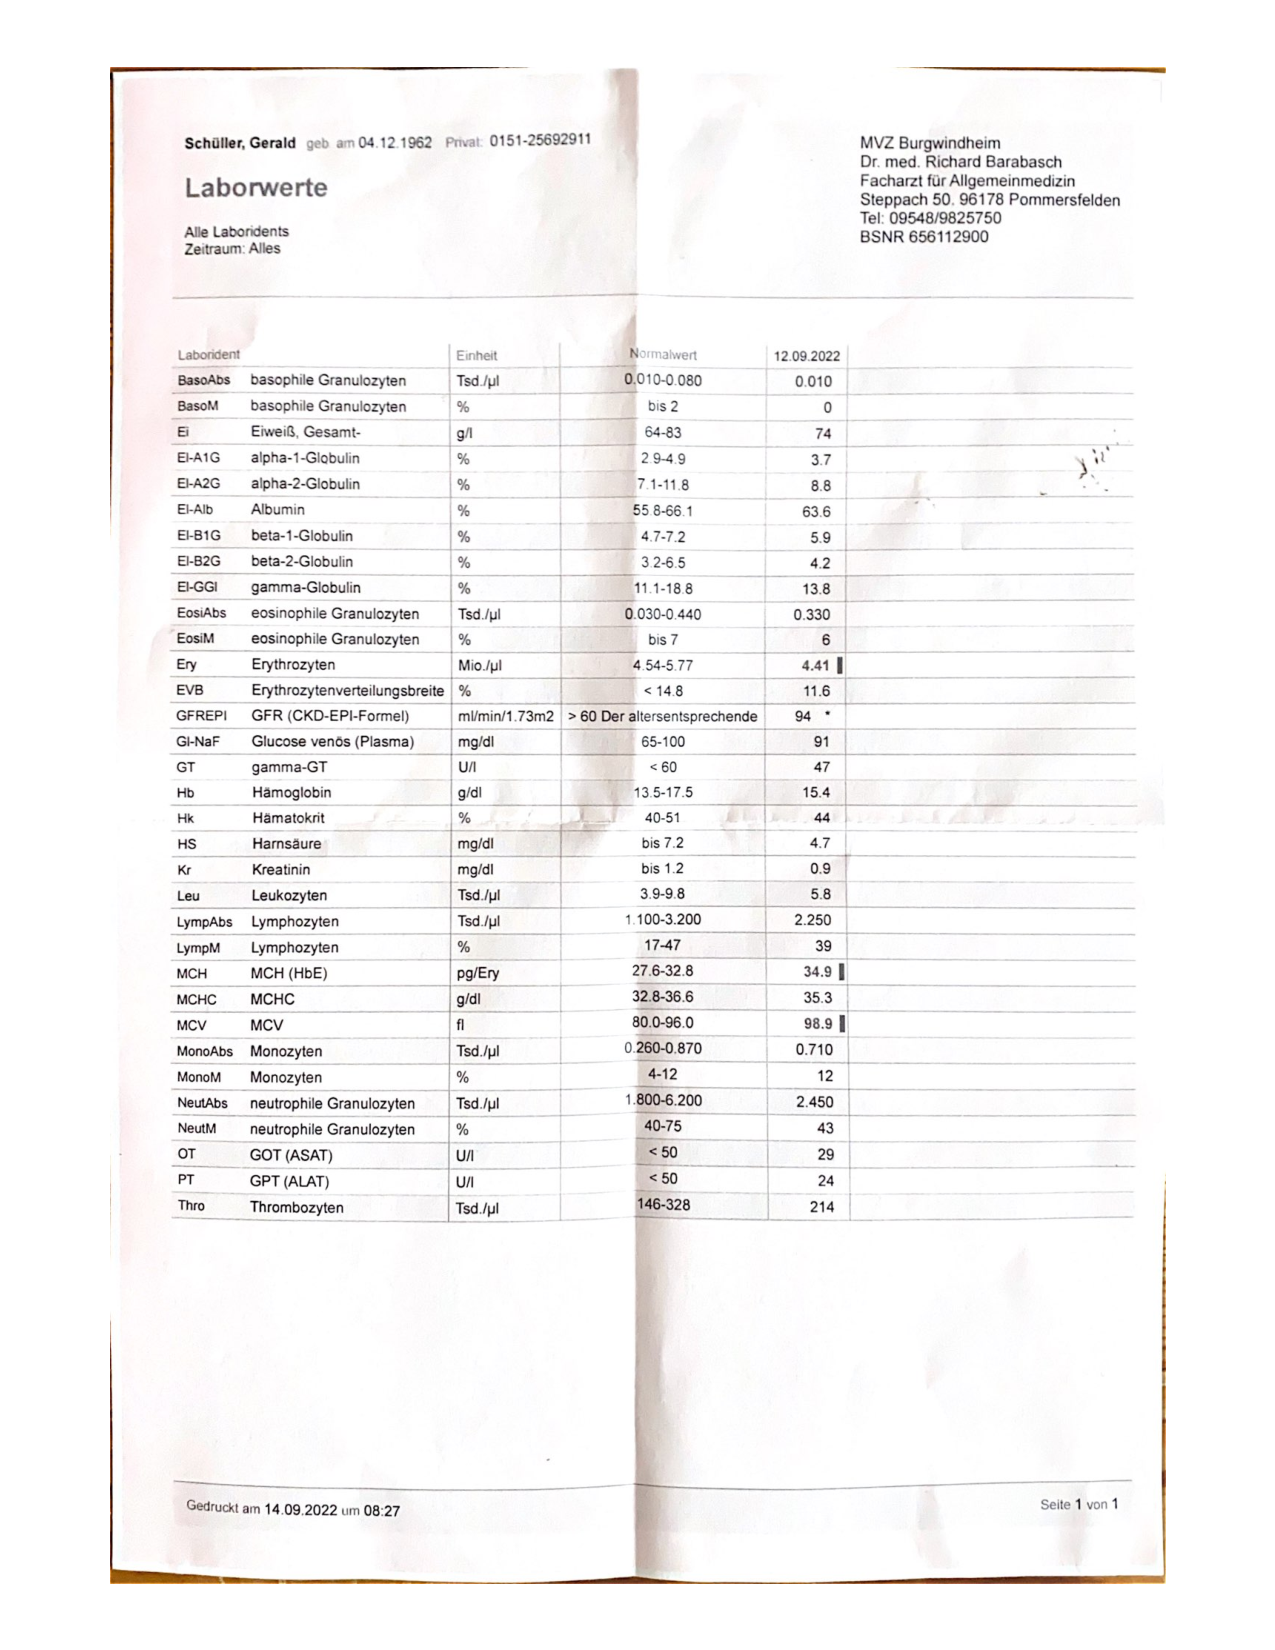
\includepdf[pages=-, scale=0.9, offset=0 0, pagecommand={%
    \begin{flushleft}  
        \section{Appendix}
      \end{flushleft} 
    \subsection{Laborwerte - 12.09.2022}\thispagestyle{plain}}
]{lw220912.pdf}

% Include the next pdf file.
% 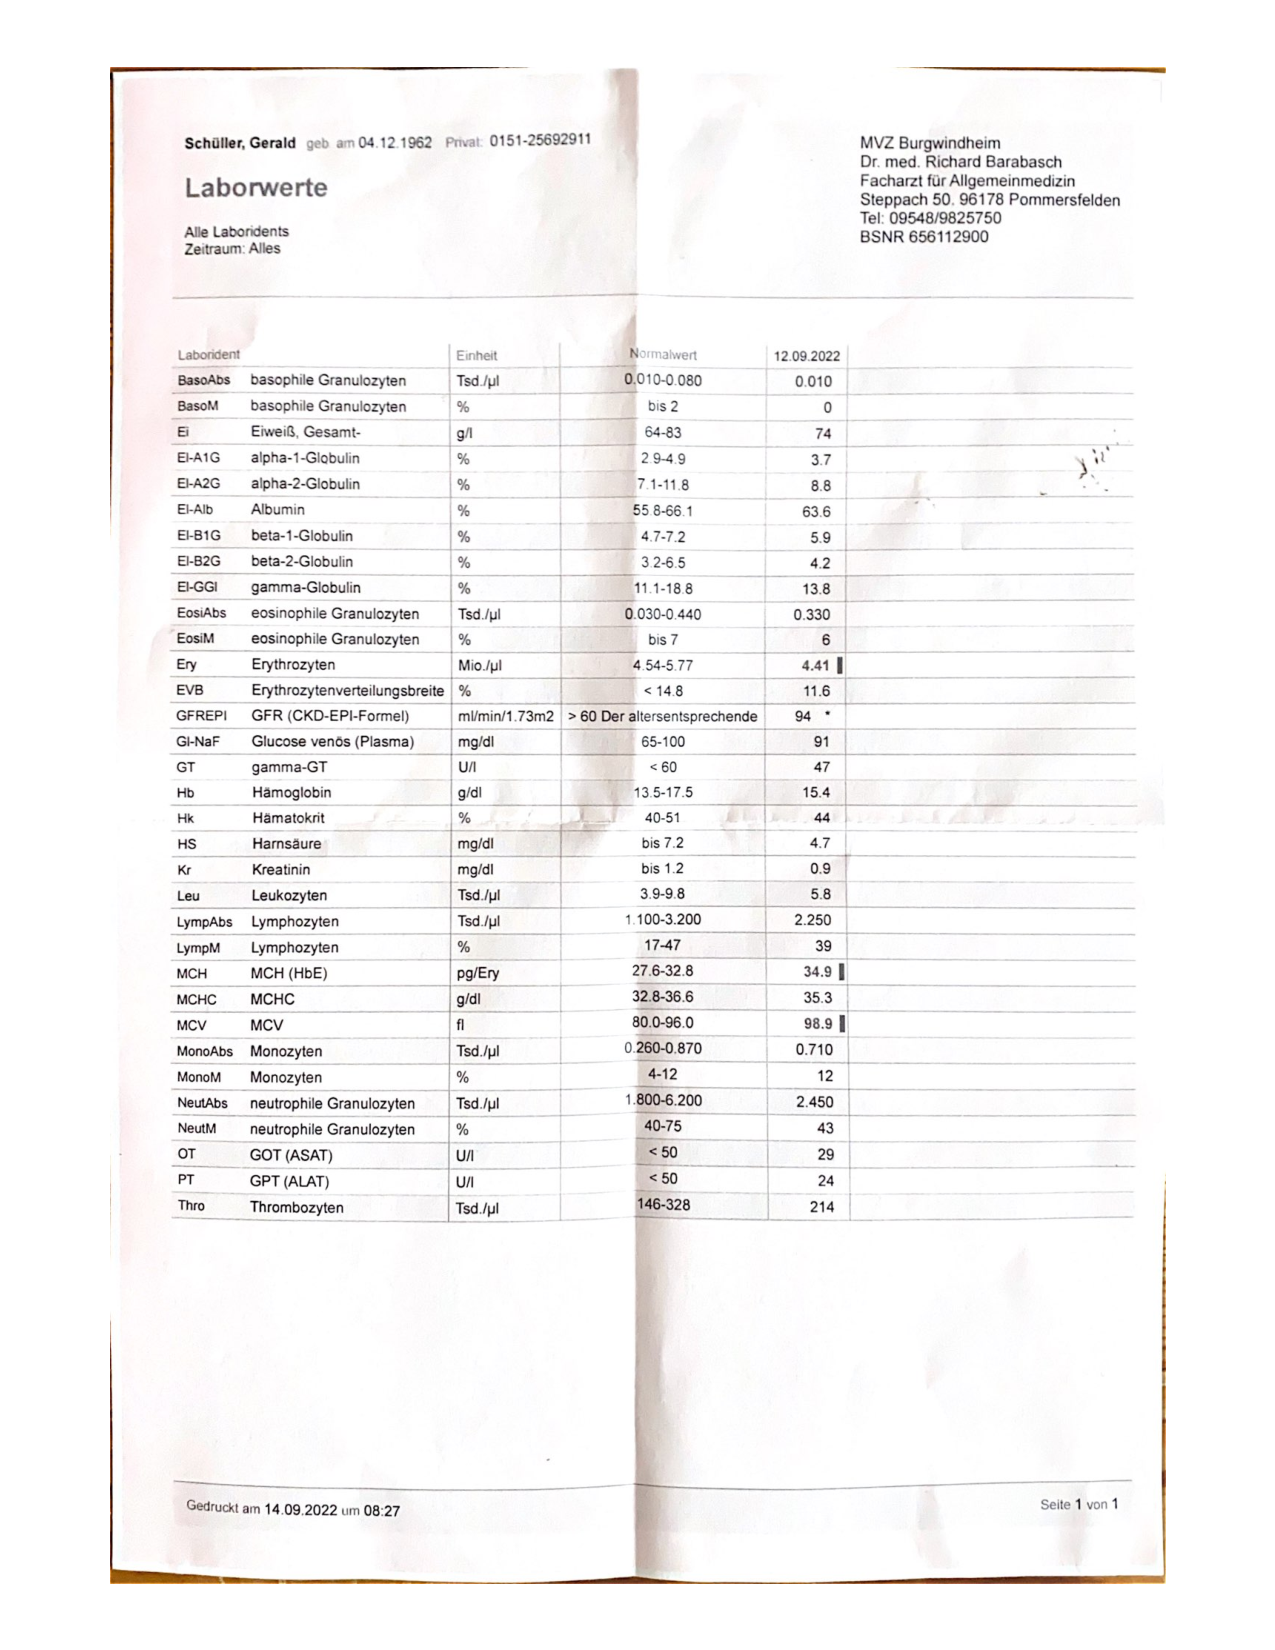
\includepdf[pages=-, scale=0.9, offset=0 0, pagecommand={%
%    \subsection{Laborwerte - 12.10.2022}\thispagestyle{plain}}
% ]{lw220912.pdf}

% End of a LaTeX text, that is to be printed.
\end{document}
